%!TEX program = lualatex
\documentclass[10pt,xcolor={dvipsnames}]{beamer}
\usetheme[
%%% options passed to the outer theme
    progressstyle=movCircCnt,   %either fixedCircCnt, movCircCnt, or corner
%    progressstyle=movCircCnt,   %either fixedCircCnt, movCircCnt, or corner
    rotationcw,          % change the rotation direction from counter-clockwise to clockwise
%    shownavsym          % show the navigation symbols
  ]{AAUsimple}
  
% If you want to change the colors of the various elements in the theme, edit and uncomment the following lines
% Change the bar and sidebar colors:
%\setbeamercolor{AAUsimple}{fg=red!20,bg=red}
%\setbeamercolor{sidebar}{bg=red!20}
% Change the color of the structural elements:
%\setbeamercolor{structure}{fg=red}
% Change the frame title text color:
%\setbeamercolor{frametitle}{fg=blue}
% Change the normal text color background:
%\setbeamercolor{normal text}{fg=black,bg=gray!10}
% ... and you can of course change a lot more - see the beamer user manual.

% \usepackage[utf8]{inputenc}
\usepackage[english]{babel}
\usepackage[T1]{fontenc}
\usepackage{epigraph}
% Or whatever. Note that the encoding and the font should match. If T1
% does not look nice, try deleting the line with the fontenc.
% \usepackage{helvet}

% colored hyperlinks
\newcommand{\chref}[2]{%
  \href{#1}{{\usebeamercolor[bg]{AAUsimple}#2}}%
}
\definecolor{colorAzulBienBonito}{RGB}{0,200,255}
\newcommand{\markdone}{\textcolor{PineGreen}{$\bullet$}}
\newcommand{\markonprogress}{\textcolor{colorAzulBienBonito}{$\bullet$}}
\newcommand{\markoff}{\textcolor{PineGreen}{$\circ$}}
\usepackage{booktabs}
\usepackage{makecell}


\usepackage{fontspec}
%%%%% CHANGING THE FONT!
\RequirePackage{etoolbox}
% \RequirePackage{ifxetex}
% \RequirePackage{ifluatex}
\RequirePackage{pgfopts}

    \setsansfont[ItalicFont={Fira Sans Light Italic},%
                 BoldFont={Fira Sans},%
                 BoldItalicFont={Fira Sans Italic}]%
                {Fira Sans Light}%
  
      \setmonofont[BoldFont={Fira Mono Medium}]{Fira Mono}%

\setbeamerfont{title}{size=\Large,%
                      series=\bfseries}
\setbeamerfont{author}{size=\small}
\setbeamerfont{date}{size=\small}
\setbeamerfont{section title}{size=\Large,%
                              series=\bfseries}
\setbeamerfont{block title}{size=\normalsize,%
                            series=\bfseries}
\setbeamerfont{block title alerted}{size=\normalsize,%
                                    series=\bfseries}
\setbeamerfont*{subtitle}{size=\large}
\setbeamerfont{frametitle}{size=\large,%
                           series=\bfseries}
\setbeamerfont{caption}{size=\small}
\setbeamerfont{caption name}{series=\bfseries}
\setbeamerfont{description item}{series=\bfseries}
\setbeamerfont{page number in head/foot}{size=\scriptsize}
\setbeamerfont{bibliography entry author}{size=\normalsize,%
                                          series=\normalfont}
\setbeamerfont{bibliography entry title}{size=\normalsize,%
                                         series=\bfseries}
\setbeamerfont{bibliography entry location}{size=\normalsize,%
                                            series=\normalfont}
\setbeamerfont{bibliography entry note}{size=\small,%
                                        series=\normalfont}
\setbeamerfont{standout}{size=\Large,%
series=\bfseries}
%%%%%%%%%%%%%%%%%%%%%%%%%%%%

\title[Smart usage of context information for the analysis, design and generation of power-aware policies for MSA's]{Smart usage of context information for the analysis, design and generation of power-aware policies for mobile sensing apps}
         
%\subtitle{Doctoral Seminar 2016}  % could also be a conference name

% \date{\today}
\date{Doctoral seminar 2016}
\author{
  Rafael Pérez Torres
  %\\\href{mailto:jkn@es.aau.dk}{{\tt jkn@es.aau.dk}}
}

% - Give the names in the same order as they appear in the paper.
% - Use the \inst{?} command only if the authors have different
%   affiliation. See the beamer manual for an example


% Dr. César Torres Huitzil Hiram Galeana Zapién, PhD
\institute[
%  {\includegraphics[scale=0.2]{aau_segl}}\\ %insert a company, department or university logo
  ITL Information Technology Laboratory\\
  Cinvestav\\
  Tamaulipas
] % optional - is placed in the bottom of the sidebar on every slide
{% is placed on the bottom of the title page
  Dr. César Torres Huitzil\\
  Dr. Hiram Galeana Zapién\\

  LTI Cinvestav
  
  %there must be an empty line above this line - otherwise some unwanted space is added between the university and the country (I do not know why;( )
}

% specify a logo on the titlepage (you can specify additional logos an include them in 
% institute command below
\pgfdeclareimage[height=1.5cm]{titlepagelogo}{AAUgraphics/aau_logo_new} % placed on the title page
%\pgfdeclareimage[height=1.5cm]{titlepagelogo2}{AAUgraphics/aau_logo_new} % placed on the title page
\titlegraphic{% is placed on the bottom of the title page
  \pgfuseimage{titlepagelogo}
%  \hspace{1cm}\pgfuseimage{titlepagelogo2}
}

\graphicspath{{../../../resources/images/}}
\begin{document}
% the titlepage
{\aauwavesbg%
\begin{frame}[plain,noframenumbering] % the plain option removes the header from the title page
  \titlepage
\end{frame}}
%%%%%%%%%%%%%%%%

% TOC
\begin{frame}{Agenda}{}
\tableofcontents
\end{frame}
%%%%%%%%%%%%%%%%

\section{Background}
\begin{frame}{Background}{Motivation}
\begin{itemize}
  \item<1-> The popularity of mobile devices is a result of advances in their computation, \textbf{sensing}, and communication dimensions~\cite{Islam2014}.
  \begin{itemize}
    \item<1-> The sensing facilities improve interaction with user, turning them into \emph{omni-sensors} able to \emph{know} about its surrounding environment.
    \item<2-> Smartphones have become \emph{context-aware} devices, gaining understanding about user's activity and environment.
    \item<3-> \textbf{Context} is the set of environmental states and settings that either determines an application's behavior or in which an application event occurs and is interesting to the user~\cite{Chen2000}.
  \end{itemize}
  \item<4-> However, battery is not evolving at the same pace than the advances in other smartphone's characteristics~\cite{Kjaergaard2012}, growing only 5-10\% each year~\cite{Ma2012,Evarts2015}.
  \begin{itemize}
    \item The energy constraint becomes critical when continuous access to sensors is needed, which is a core requirement of \textbf{mobile sensing applications}. 
  \end{itemize}
\end{itemize}
\end{frame}

\begin{frame}{Background}{Stages of mobile sensing applications}
\begin{figure}%[tb]
  \centering
  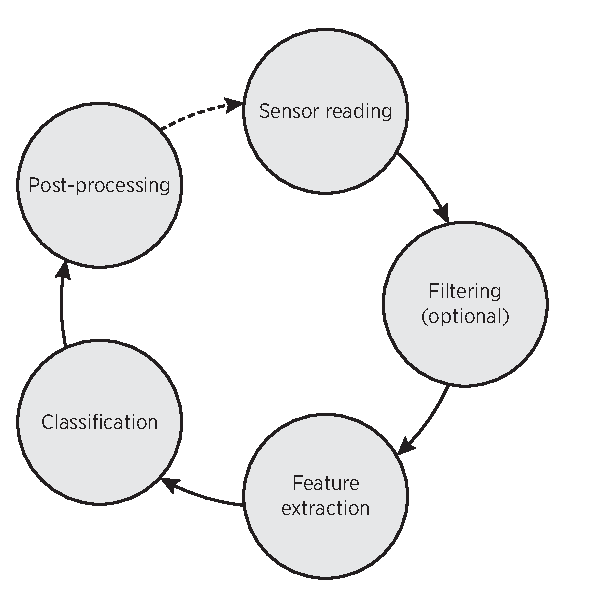
\includegraphics[width=\textwidth]{vectors/msa-stages}
  \caption{Stages of mobile sensing applications}
  \label{fig:msa-stages}
\end{figure}
There is a tradeoff between the accuracy of context information retrieved and the associated energy consumption~\cite{Sim2014,Rachuri2012}.
How to face it?
\end{frame}

\section{Problem statement}
\begin{frame}{Problem definition}{Hypothesis}
\begin{exampleblock}{Hypothesis}
Intelligent policies produced through context information built from sensors data could be employed to reduce the energy consumption in a mobile device when performing continuous sensor readings.
\end{exampleblock}
%\pause
{
\small
\pause
\begin{itemize}
  \item An intelligent policy is a special rule that defines how sensors should be selected and configured to reduce energy consumption and achieve the mobile sensing app's requirements.
  It is intelligent in terms of self-adaptness to changes detected in context information across time.
  \pause
  \item This research work is aimed at employing GPS and inertial sensors data (accelerometer) for inferring context information in terms of mobility patterns.
  This context information will then be exploited to adapt sensors' operation and produce power savings.
\end{itemize}
}
\end{frame}

\begin{frame}{Problem definition}{Problem statement}
\begin{alertblock}{Problem 1: Mobility pattern identification}
\small
Given a set $V = \left\{v_{1}, v_{2}, \dotsc, v_{n}\right\}$ of data values read from sensor $S$ in the time interval $T  \in [t_{1}, t_{2}]$, identify the current mobility pattern $p_{S}$ that represents the activity of user.

\begin{equation}
  \text{PatternIdentifier}( V ) \longrightarrow{} p_{S} \in \text{\textbf{Patterns}}
\end{equation}

Where $\text{\textbf{Patterns}}$ is a set of patterns that represent a user's mobility context situation, specifically the set \scriptsize{\texttt{ \{no movement, walking, running, vehicle transportation, arriving stay point, leaving stay point\} }}.
\pause
\begin{figure}[tb]
  \centering
  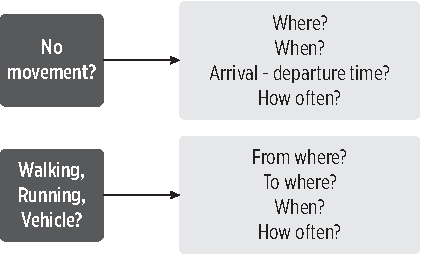
\includegraphics[scale=0.55]{vectors/mobility-patterns-implications}
  \caption{Context information related to mobility patterns}
  \label{fig:mobility-patterns-implications}
\end{figure}
\end{alertblock}
\end{frame}

\begin{frame}{Problem definition}{Problem statement}
\begin{alertblock}{Problem 2: Policy generation}
\small
Given the set of detected mobility patterns $\mathcal{P} = \{ p_{S_1}, p_{S_2}, \ldots, p_{S_n} \}$ in data from sensors $\mathcal{S} = \{ S_1,S_2,\ldots, S_n \}$, accuracy required $a$, and physical constraints status $c$ of a mobile device, find a policy that select the proper set of sensors $\mathcal{S}_{new}$ and its associated configuration $\mathcal{S}_{new_{conf}}$  while meeting application requirements.

\begin{equation}
  \text{PolicyGeneration}( \mathcal{P}, a, c ) \longrightarrow{} \mathcal{S}_{new}, \mathcal{S}_{new_{conf}}
\end{equation}

The $\mathcal{S}_{new_{conf}}$ configuration is referred to as the \emph{adaptive duty cycle} of associated sensors.
\end{alertblock}
\end{frame}

\begin{frame}{Problem definition}{Interaction between problems}
\begin{figure}[tb]
  \centering
  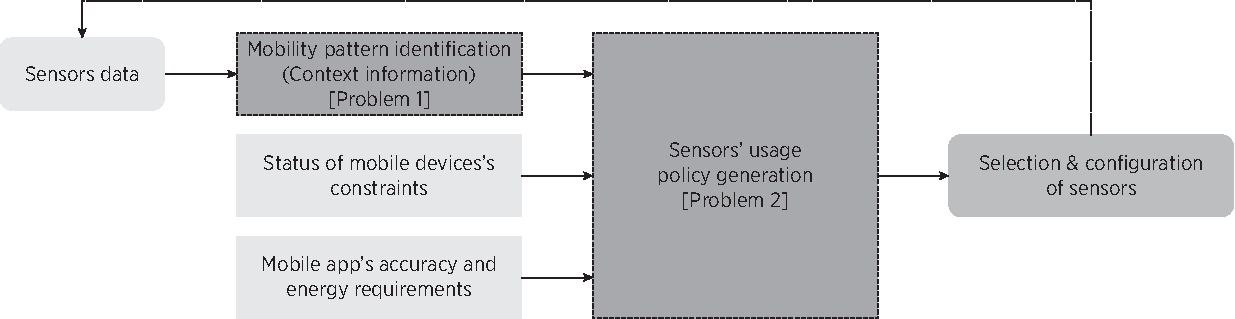
\includegraphics[width=\textwidth]{../../../resources/images/vectors/problems-incorporation}
  \caption{Interaction between problems}
  \label{fig:problems-incorporation}
\end{figure}
\end{frame}

\begin{frame}{Problem definition}{Objectives}
\begin{exampleblock}{Main objective}
To reduce energy consumption in the mobile sensing apps, which perform continuous sensor readings, through self-adapting power-aware policies generated from context information obtained from sensors data.
\end{exampleblock}
\pause
\begin{exampleblock}{Particular objectives}
\small
\begin{itemize}
  \item To identify mobility patterns from context information obtained from an inertial sensor (accelerometer) and location providers (GPS).
  \pause
  \item To generate an accurate representation of mobility patterns, which in conjunction with accuracy mobile app requirements and mobile device constraints, allows to generate power-aware GPS sensing policies.
  \pause
  \item To reduce energy consumption in location-based mobile sensing apps through a middleware that implements policies fed with mobility patterns learned from sensors data.
\end{itemize}
\end{exampleblock}
\end{frame}

\begin{frame}{Problem definition}{Expected contributions}
\begin{itemize}
  \item<+-> A mechanism for detecting mobility patterns from the data read by sensors of mobile devices (GPS and accelerometer).
  \item<+-> A mechanism for generating policies for accessing sensors.
  The produced policies will allow to perform an intelligent usage of smartphone's sensing facilities in continuous sensor sampling, reducing the energy consumption.
  \item<+-> A middleware implementing the previous power-aware mechanisms for easing the development of location based services.
\end{itemize}
\end{frame}

\begin{frame}{Problem definition}{Problem's scenario}
\begin{figure}
  \centering
  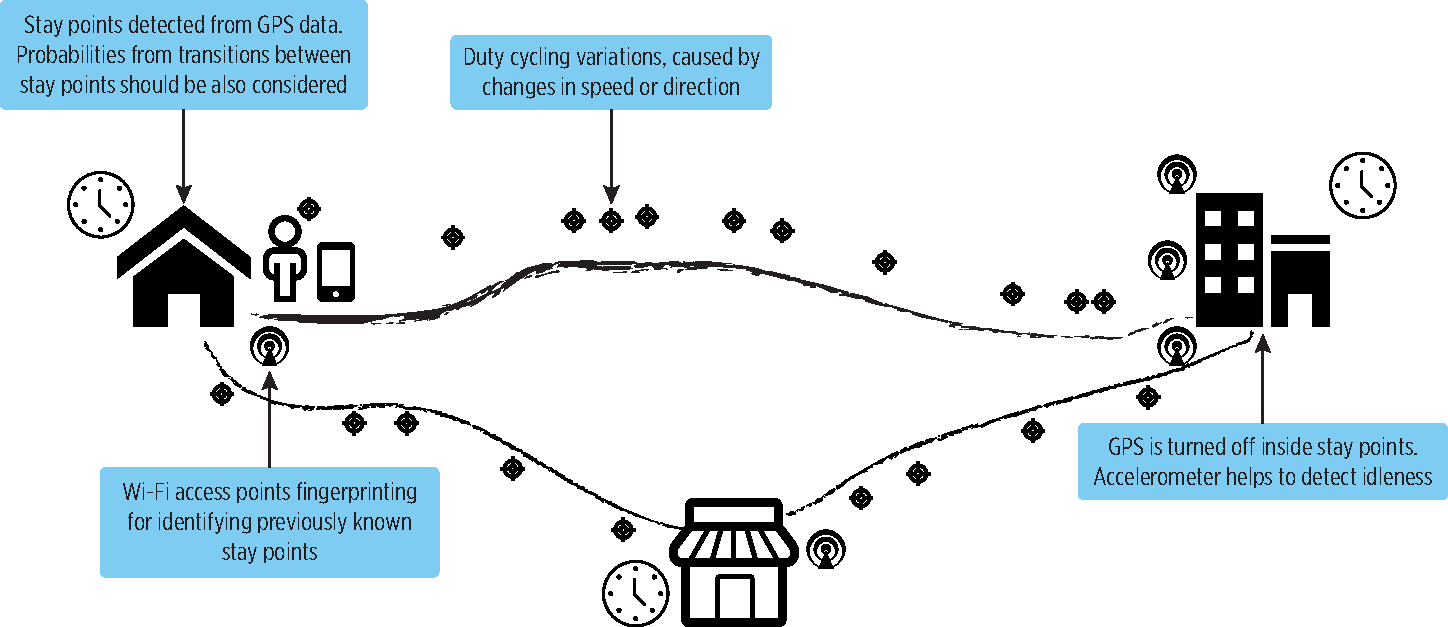
\includegraphics[width=\textwidth]{vectors/scenario}
  \caption{Basic problem's scenario}
  \label{fig:scenario}
\end{figure}
\end{frame}

\section{Related work}
\begin{frame}{Related work}{Previous work}
\begin{figure}
  \centering
  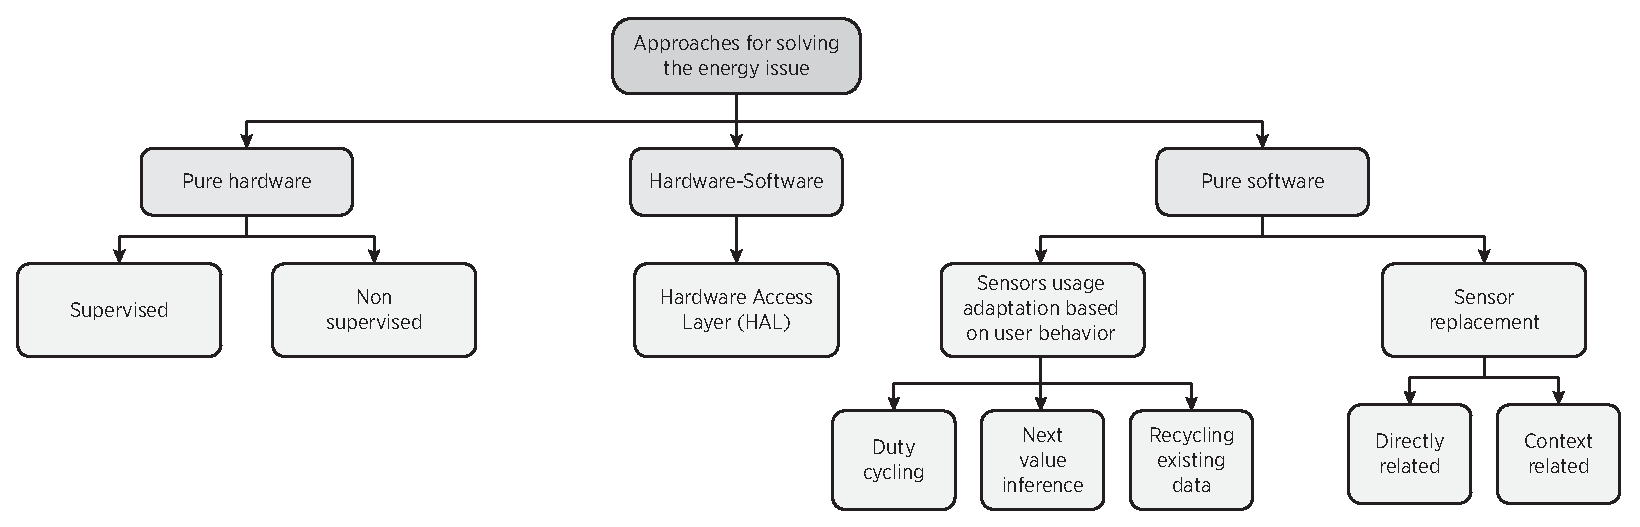
\includegraphics[width=\textwidth]{../../../resources/images/vectors/approaches-taxonomy}
  \caption{Taxonomy of related work solutions}
  \label{fig:taxonomy}
\end{figure}
\end{frame}


\section{Methodology}
\begin{frame}{Methodology}{Methodology steps}
\begin{enumerate}
  \item \textbf{Familiarization with state-of-art power-aware sensing related techniques}
  \item \textbf{Formal definition and selection of mobility patterns to be identified}
  \item \textbf{Research on pattern recognition algorithms focused on mobility patterns identification}
  \item \textbf{Design of the Pattern Identification Element (PIE)}
  \item \textbf{Research on (and proposition of) adaptive policies for energy efficient usage of sensors}
  \item Design of the Policy Generation Element (PGE)
  \item Development of a middleware involving the PIE and PGE for the Android platform
  \item Experimentation in terms of accuracy and energy efficiency
\end{enumerate}
\end{frame}

\section{Proposed solution}
\begin{frame}{Proposed solution}{Characteristics}
\begin{itemize}
  \item Pure software approach.
  \pause
  \item Event-driven oriented, completely on device.
  \begin{itemize}
    \item Top level mobility states-events: \texttt{on trajectory}, \texttt{on stay point}.
    \pause
    \item Low level mobility states-events: \texttt{transportation mode changed}, \texttt{arriving to stay point}, \texttt{leaving stay point}.
    \pause
  \end{itemize}
  \item Inspired on Cognitive Dynamic Systems~\cite{Haykin2006}, including 
  \begin{itemize}
    \item Perception-action cycle.
    \pause
    \item Memory.
    \pause
    \item Attention.
    \pause
    \item Intelligence.
  \end{itemize}
\end{itemize}
\end{frame}

\begin{frame}{Proposed solution}{Overview}
\begin{figure}
  \centering
  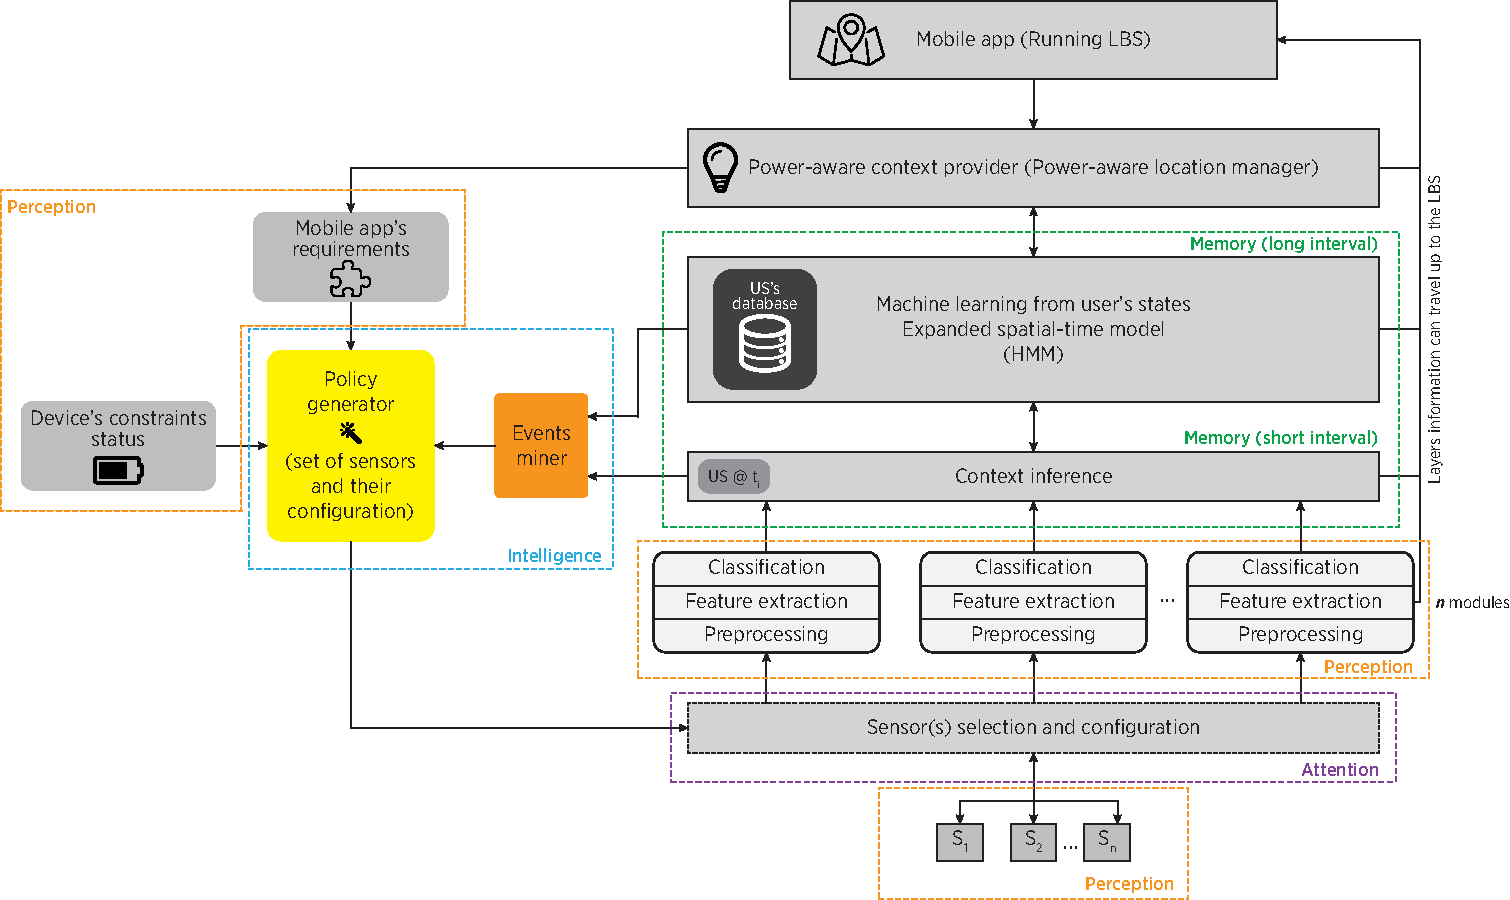
\includegraphics[width=0.9\textwidth]{vectors/solution-general-overview}
  \caption{Overview of current solution}
  \label{fig:solution}
\end{figure}
\end{frame}

\begin{frame}{Proposed solution}{Operation}
\begin{itemize}
  \item Overall problem divided into:
  \begin{itemize}
    \item Detection of stay points (The anchor points that user visits frequently).
    \pause
    \item Tracking of user commuting between stay points (Transition probability).
  \end{itemize}
\end{itemize}
\pause
\begin{figure}
  \centering
  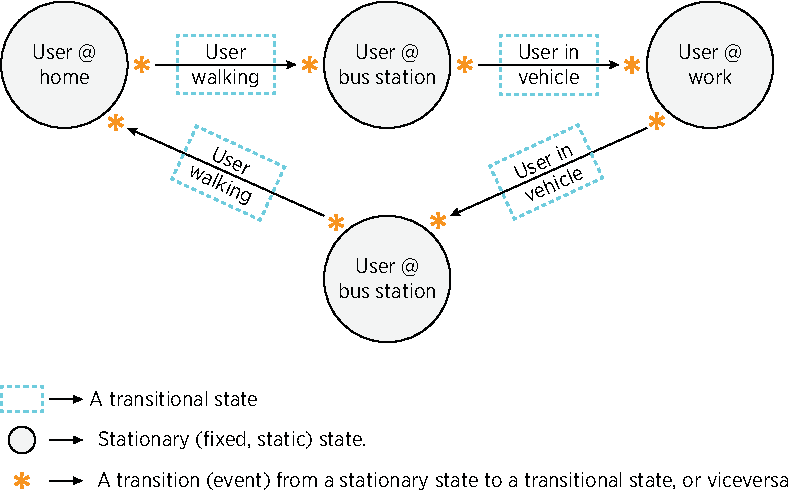
\includegraphics[width=0.55\textwidth]{vectors/zoom-expanded-spatial-time-model}
  \caption{Information modeled by the expanded spatial-time model}
  \label{fig:information-modeled-spatial-time-model}
\end{figure}
\end{frame}

\section{Schedule}
\begin{frame}{Schedule}
\begin{table}[]
\centering
\resizebox{0.95\textwidth}{!}{%
\begin{tabular}{clccccccc}
   &                                                                               & 2014 & \multicolumn{3}{c}{2015} & \multicolumn{3}{c}{2016}  \\
   \cline{3-9}
\multicolumn{2}{l}{\small{Work: \markdone~Done, \markonprogress~In progress, \markoff~To be done}} & 3rd & 1st & 2nd & 3rd & 1st & 2nd & 3rd \\
   \toprule
\multicolumn{2}{c}{\textsc{Step I}}                                                &  &  &  &  &  &  &  \\
1  & State-of-art reading                                                          & \markdone & \markdone &  &  &  &  &  \\
2  & State-of-art works categorization                                             &  & \markdone & \markdone  &  &  &  &  \\
3  & Documentation of information found (committee request)                        &  &  & \markdone &  &  &  &  \vspace{1em}\\

\multicolumn{2}{c}{\textsc{Step II}}                                               &  &  &  &  &  &  &  \\
4  & \makecell[l]{Development of a mobile app for accelerometer and location \\data collection}    &  &  & \markdone & \markdone  &  &  &  \\
5  & Analysis of data                                                              &  &  &  & \markdone  &  &  &  \\
6  & Formal definition of mobility pattern                                         &  &  &  & \markdone &  &  &  \\
7  & Selection of mobility patterns                                                &  &  &  & \markdone & \markdone &  &  \vspace{1em}\\

\multicolumn{2}{c}{\textsc{Step III}}                                              &  &  &  &  &  &  &  \\
8  & Research on classification algorithms for mobility patterns                   &  &  &  & \markdone & \markdone &  &  \\
9  & Definition of metrics for evaluating algorithms                               &  &  &  &  & \markdone &  &  \\
10 & Implementation of algorithms in mobile platform                               &  &  &  &  & \markdone & \markdone  &  \\
11 & Selection of best algorithms according to metrics                             &  &  &  &  &  & \markdone &  \vspace{1em}\\

\multicolumn{2}{c}{\textsc{Step IV}}                                               &  &  &  &  &  &  &  \\
12 & Definition and modeling of parameters needed by the PIE                       &  &  &  & \markdone & \markdone & \markdone & \markonprogress \\
13 & Building of the PIE                                                           &  &  &  & \markdone & \markdone & \markdone & \markonprogress \\
\bottomrule
\end{tabular}%
}
\caption{Schedule of activities (each column represents a four months period)}
\label{tbl:schedule-part-one}
\end{table}
\end{frame}

\begin{frame}{Schedule}
\begin{table}[]
\centering
\resizebox{0.95\textwidth}{!}{%
\begin{tabular}{clccccccc}
   &                                                                               & \multicolumn{3}{c}{2016} & \multicolumn{3}{c}{2017} & 2018 \\
   \cline{3-9}
\multicolumn{2}{l}{\small{Work: \markdone~Done, \markonprogress~In progress, \markoff~To be done}}   & 1st & 2nd & 3rd & 1st & 2nd & 3rd & 1st \\
   \toprule
\multicolumn{2}{c}{\textsc{Step V}}                                                &  &  &  &  &  &  & \\
14  & Formal definition of policy                                                  &  &  & \markdone &  &  &  & \\
15  & \makecell[l]{Research and evaluation of techniques for\\generation and adaption of policies}&  &  & \markonprogress & \markonprogress  &  &  & \\
16  & Design and execution of experiments applied to use cases                     &  &  & \markonprogress & \markonprogress  &  &  & \\
17  & Selection of policies                                                        &  &  &  & \markonprogress  &  &  & \vspace{1em} \\

\multicolumn{2}{c}{\textsc{Step VI}}                                               &  &  &  &  &  &  & \\
18  & Definition and modeling of PGE parameters                                    &  &  &  &  & \markonprogress  &  & \\
19  & Building of the PGE                                                          &  &  &  &  & \markonprogress  &  & \vspace{1em} \\

\multicolumn{2}{c}{\textsc{Step VII}}                                               &  &  &  &  &  &  & \\
20  & Analysis of components into software abstractions                             &  &  &  &  & \markonprogress  &  & \\
21  & Research on Android API for specialized components                            &  &  &  &  & \markonprogress  &  & \\
22  & Development of middleware                                                     &  &  &  &  & \markonprogress  &  & \vspace{1em}\\

\multicolumn{2}{c}{\textsc{Step VIII}}                                              &  &  &  &  &  &  & \\
23  & \makecell[l]{Definition of experiments aimed at accuracy\\and energy consumption metrics}    &  &  &  &  &  & \markoff & \\
24  & Development of experimental sample mobile apps                                &  &  &  &  &  & \markoff & \\
25  & Experiments execution                                                         &  &  &  &  &  & \markoff & \markoff  \\
26  & Final results analysis                                                              &  &  &  &  &  &  & \markoff \\
\bottomrule
\end{tabular}%
}
\caption{Schedule of activities (each column represents a four months period)}
\label{tbl:schedule-part-two}
\end{table}
\end{frame}

\begin{frame}{Schedule}
\begin{table}
\centering
\resizebox{\textwidth}{!}{%
\begin{tabular}{clcccccccccccc}
   &                                                                               & 2014 & \multicolumn{3}{c}{2015} & \multicolumn{3}{c}{2016} & \multicolumn{3}{c}{2017} & \multicolumn{2}{c}{2018} \\
   \cline{3-14}
 \multicolumn{2}{l}{\small{Work: \markdone~Done, \markonprogress~In progress, \markoff~To be done}} & 3rd & 1st & 2nd & 3rd & 1st & 2nd & 3rd & 1st & 2nd & 3rd & 1st & 2nd\\
   \toprule
\multicolumn{2}{c}{\textsc{Required tasks}}                                        &  &  &  &  &  &  &  &  &  &  &  & \\
A   & Related courses                                                              & \markdone  & \markdone  & \markdone &  &  &  &  &  &  &  &  & \\
B   & Research articles submission                                                 &  &  &  & \markdone &  & \markdone &  &  &  &  & \markoff & \\
C   & Predoctoral exam preparation                                                 &  &  &  &  &  &  &  &  & \markoff &  &  & \\
D   & Thesis writing                                                               & \markdone  &  &  & \markdone &  &  & \markonprogress &  &  & \markoff & \markoff & \markoff \\

\bottomrule
\end{tabular}%
}
\caption{Schedule of required activities}
\label{tbl:schedule-required-activities}
\end{table}
\end{frame}



% \begin{frame}{Schedule (Option B)}
% \begin{table}
% \small
% \centering
% \resizebox{0.98\textwidth}{!}{%
% \begin{tabular}{clcccccccccccc}
%    &                                                                               & 2014 & \multicolumn{3}{c}{\small{2015}} & \multicolumn{3}{c}{\small{2016}} & \multicolumn{3}{c}{\small{2017}} & \multicolumn{2}{c}{\small{2018}} \\
%    \cline{3-14}
% \multicolumn{2}{l}{\scriptsize{Work: \markdone~Done, \markonprogress~In progress, \markoff~To be done}} & \scriptsize{3rd} & \scriptsize{1st} & \scriptsize{2nd} & \scriptsize{3rd} & \scriptsize{1st} & \scriptsize{2nd} & \scriptsize{3rd} & \scriptsize{1st} & \scriptsize{2nd} & \scriptsize{3rd} & \scriptsize{1st} & \scriptsize{2nd}\\
%    \toprule
% \multicolumn{2}{c}{\textsc{Methodology steps}}                                                               &  &  &  &  &  &  &  &  &  &  &  & \\
% 1   & \makecell[l]{Familiarization with state-of-art power-aware \\sensing related techniques}               & \markdone  & \markdone  & \markdone &  &  &  &  &  &  &  &  & \vspace{0.25em}\\
% 2   & \makecell[l]{Formal definition and selection of mobility \\patterns to be identified}                  &  &  & \markdone & \markdone & \markdone &  &  &  &  &  &  & \vspace{0.25em}\\
% 3   & \makecell[l]{Research on pattern recognition algorithms \\focused on mobility patterns identification} &  &  &  & \markdone & \markdone & \markdone &  &  &  &  &  & \vspace{0.25em}\\
% 4   & \makecell[l]{Design of the Pattern Identification Element (PIE)}                                       &  &  &  & \markdone & \markdone & \markdone & \markonprogress &  &  &  &  &  \vspace{0.25em}\\
% 5   & \makecell[l]{Research on (and proposition of) adaptive \\policies for energy efficient usage of sensors} &  &  &  &  &  &  & \markonprogress & \markonprogress &  &  &  & \vspace{0.25em}\\
% 6   & \makecell[l]{Design of the Policy Generation Element (PGE)}                                            &  &  &  &  &  &  &  &  & \markonprogress &  &  &  \vspace{0.25em}\\
% 7   & \makecell[l]{Development of a middleware implementing \\the PIE and PGE for the Android platform}            &  &  &  &  &  &  &  &  & \markonprogress &  &  &  \vspace{0.25em}\\
% 8   & \makecell[l]{Experimentation in terms of accuracy and \\energy efficiency}                                  &  &  &  &  &  &  &  &  &  & \markoff & \markoff & \vspace{1em} \\

% \multicolumn{2}{c}{\textsc{Required tasks}}                                        &  &  &  &  &  &  &  &  &  &  &  & \\
% A   & Related courses                                                              & \markdone  & \markdone  & \markdone &  &  &  &  &  &  &  &  & \vspace{0.2em} \\
% B   & Research articles submission                                                 &  &  &  & \markdone &  & \markdone &  &  &  &  & \markoff & \vspace{0.25em} \\
% C   & Predoctoral exam preparation                                                 &  &  &  &  &  &  &  &  & \markoff &  &  & \vspace{0.2em} \\
% D   & Thesis writing                                                               & \markdone  &  &  & \markdone &  &  & \markonprogress &  &  & \markoff & \markoff & \markoff \\
% \bottomrule
% \end{tabular}%
% }
% \caption{Schedule of methodology activities}
% \label{tbl:schedule-required-activities-summarized}
% \end{table}
% \end{frame}

\section{Conclusions}
\begin{frame}{Conclusions}{}
As conclusions, the current talk has been provided:
\begin{itemize}
  \item<+-> The antecedents and motivation of the current research.
  \item<+-> A methodology based on the usage of context information for reducing energy consumption in location-based mobile apps.
  \item<+-> The main blocks of a middleware with an event-driven design and Cognitive Dynamic Systems fundamentals.
  \item<+-> The detailed work plan for addressing each of the methodology steps, including performed and pending activities.
\end{itemize}
\end{frame}

{\aauwavesbg
\begin{frame}[plain,noframenumbering]
  \finalpage{
    Thank you for your attention!
  }
  { \tiny
    \epigraph{\tiny We make our world significant by the courage of our questions and by the depth of our answers.}{\tiny \textit{Carl Sagan}}
  }
\end{frame}}

\begin{frame}[allowframebreaks]
        \frametitle{References}
%\bibliographystyle{plain}
\bibliographystyle{unsrt}
\bibliography{../../../../../resources/references/library}
\end{frame}

\end{document}
